% $Id: calculations-jets.tex 527 2019-10-22 15:29:52Z smarzani $
%
% This contains basic calculations for jet physics, in particulwar the
% jet mass at fixed order and resummed
%------------------------------------------------------------------------
\chapter{Calculations for jets: the jet mass distribution}\label{chap:calculations-jets}
%
In this chapter we begin our discussion about the calculation of jet properties in perturbative QCD.
%
We start by considering  an important observable in jet physics, namely the jet invariant mass
\begin{equation}\label{eq:jet-mass-def}
m^2=\bigg( \sum_{i \in \text{jet}}k_i\bigg)^2,
\end{equation}
where the sum runs over all the particles $i$ which are clustered in the jet. 
%
In this lecture notes, because of its simple definition, we are going to take the jet mass as the prototype of a jet substructure observable.
%
This observable will be discussed in detail in this
  chapter and we will again come back to it in
  Chapter~\ref{calculations-substructure-mass} where we are going to compute the jet
  mass for jets modified by substructure techniques, a case
  particularly relevant for phenomenological applications at the
  LHC.
  %

In our discussion, we shall focus on QCD jets, i.e.\ jets which are initiated by a hard parton and subsequently evolve through parton shower. 
%
%
Our perturbative analysis will mostly performed at parton level, i.e.\
we will consider quarks and gluons to be the jet's
constituents. Perturbation theory is not able to describe the
transition to particle level and hadronisation models are usually
employed in event generators to describe the parton-to-hadron
transition.  In this chapter, we will only briefly comment on these
non-perturbative issues, postponing a numerical analysis of their impact to Chapter~\ref{calculations-substructure-mass}.
%
Even if we remain within the regime of perturbative QCD, we will see
that the fixed-order methods are not adequate in order to capture the
relevant dynamics of the jet mass, especially in the boosted regime
where emissions are accompanied by large logarithms. Thus, we will
exploit all-order resummation techniques to better handle the theoretical description of this observable.
%
%
In order to maintain our presentation as simple as possible, while discussing most of the relevant features, we are going to still focus our discussion on jets produced in $e^+e^-$. 
%
We shall comment on the complication that arise when considering hadron-hadron collisions in Sec.~\ref{sec:pp-collisions}.
%
In order to make the connection between the $e^+e^-$ and the $pp$ discussion as close as possible, we consider in both cases jets clustered with a generalised $k_t$ algorithm with radius $R$, in its $e^+e^-$ and $pp$ adaptations, respectively~\cite{Cacciari:2011ma}.

\section{The one-loop calculation}
We start by considering the so-called cumulative distribution, which is defined as the normalised cross-section for measuring a value of the jet mass below a certain $m^2$:
\begin{equation}\label{eq:cumu-def}
\Sigma(m^2)= \frac{1}{\sigma_0}\int_0^{m^2} d {m'}^2 \frac{d \sigma}{d {m'}^2}=1+\as \Sigma^{(1)}+\ord \left( \as^2\right),
\end{equation}
where following common practice in the literature, we have chosen to use the Born cross-section as a normalisation factor. The cumulative distribution is a dimensionless quantity and so we can anticipate that its dependence on the jet mass must come as a ratio to another energy scale, which is typically the jet energy (or in proton-proton collision the jet transverse momentum).

We first tackle the calculation of Eq.~(\ref{eq:cumu-def}) to $\ord
\left(\as \right)$, in the soft limit. Thus, we consider the eikonal
factor for the quark-antiquark dipole (cf.~Eq.~(\ref{eq:real-virtual-together}))
\begin{align}\label{eq:dipole-quark-antiquark}
W_{12}&= \frac{\as}{2 \pi} (2 C_F) \frac{k_1 \cdot k_2}{(k_1 \cdot k_3)(k_2 \cdot k_3)},
\end{align}
where $k_1$ and $k_2$ are the momenta of the quark and antiquark respectively and $k_3$ is the momentum of the soft gluon. For instance, we can choose to parametrise them as
\begin{align}
k_1&=\frac{Q}{2} \left(1,0,0,1 \right), \quad k_2=\frac{Q}{2} \left(1,0,0,-1 \right), \nonumber\\
k_3&= \omega \left(1, \sin \theta \cos \phi, \sin \theta \sin \phi, \cos \theta \right).
\end{align}
In terms of the above parametrisation of the kinematics, the Lorentz-invariant phase-space becomes
\begin{equation}\label{eq:phase-space-integration}
\int d\Phi\equiv \int_0^\infty \omega\, d\omega \int_{-1}^1 d\cos \theta \int_0^{2\pi}\frac{d\phi}{2\pi}.
\end{equation}
This is equivalent to $\tfrac{1}{\pi}\int d^4k_3\delta(k_3^2)$, which
for simplicity has a slightly different normalisation convention
than Eq.~(\ref{eq:4vect-phase-space}).\footnote{Watch out that
  different conventions are present in the literature. For example
  (see \eg~\cite{Dasgupta:2007wa}), one sometimes uses
  $\int d^4k_3\delta(k_3^2)$ as a phase-space integration, in which
  case Eq.~\eqref{eq:dipole-quark-antiquark} has a
  $\tfrac{\alpha_s}{2\pi^2}$ factor instead of
  $\tfrac{\alpha_s}{2\pi}$.}  Note that in the above expression we are
allowed to ignore any recoil of the quarks against the gluon because
we work in the soft limit. Furthermore, in this limit, the energy of
the jet is simply $Q/2$.
%
The colour factor $2 C_F$ in Eq.~(\ref{eq:dipole-quark-antiquark})
emerges because we are in the presence of only one dipole. For a
process with more hard partonic lines, we should sum over all possible
dipoles each of which is accompanied by the effective colour factors
introduced in Eq.~(\ref{eq:eff-col-def}).


The one-loop evaluation of the cumulative distribution is then obtained adding together real and virtual corrections. At one loop these contributions are both given by the eikonal factor $W_{12}$, but with opposite sign. Another crucial difference is that when the emitted gluon is real, then we have to impose the appropriate phase-space constraints. 
%
In particular, if the gluon is clustered in the jet seeded by the hard parton $k_1$, then its contribution to the jet mass is constrained to be less than $m^2$. 
%
If instead it falls outside the jet, then it only contributes to the zero-mass bin. 
%
In formulae, we have~\footnote{For simplicity, we introduce the
  following notation for the Heaviside step function:
  $\Theta\left( a>b\right)\equiv \Theta\left( a-b\right)$,
  $\Theta\left( a<b\right)\equiv \Theta\left( b-a\right)$, and
  $\Theta\left( a<b<c\right)\equiv \Theta\left(b-a \right)
  \Theta\left(c-b \right)$.  }
\begin{align}\label{eq:sigma-1-loop-begin}
\as \Sigma^{(1)}(m^2)&=\int_{-1}^1 d \cos \theta \int_0^{2 \pi} \frac{d \phi}{2 \pi} \int_0^{Q/2} \omega d \omega
\frac{2 C_F \as}{\pi} \frac{1}{\omega^2 (1-\cos \theta)(1+\cos \theta)} 
\nonumber \\ & \times
\left[ \Theta_\text{in jet} \Theta \left(2\frac{Q \omega}{2}(1-\cos \theta) < m^2 \right)
+\Theta_\text{out jet} -1\right]\nonumber\\
&= - \frac{2 \as C_F}{\pi} \int_{\cos R}^{1- 2 \frac{m^2}{Q^2}} 
\frac{d \cos \theta }{(1-\cos \theta)(1+\cos \theta)} \log\left( \frac{Q^2 (1- \cos \theta)}{2 m^2}\right),
\end{align}
In the above equation, we have used $\Theta_\text{in jet}=\Theta\left(1-\cos \theta< 1-\cos R \right)$ and $\Theta_\text{out jet}=1-\Theta_\text{in jet}$ , which, for a jet made up of two particles, is the condition to be satisfied for any clustering algorithm of the generalised $k_t$ family. We will see in Sec.~\ref{sec:clustering} that beyond one loop the details of the clustering algorithm affect the single-logarithmic structure of the jet mass distribution.

The integral over the gluon angle is fairly straightforward. Since we
are interested in the logarithmic region, we neglect powers of the jet
mass divided by the hard scale $Q$:
\begin{align}\label{eq:sigma-1-loop-cntd}
\as \Sigma^{(1)}&=- \frac{\as C_F}{2 \pi} 
\left[\log^2 \left( \frac{Q^2}{m^2}\tan^2 \frac{R}{2} \right) -\log^2 \left(\cos^2 \frac{R}{2}\right)- 2 \text{Li}_2\left(\sin^2\frac{R}{2} \right) \right] +\ord \left(\frac{m^2}{Q^2} \right),
\end{align}
which is valid for $\frac{m^2}{Q^2}< \sin^2\frac{R}{2}$.
Thus, we see that the jet mass distribution exhibits a double
logarithmic behaviour in the ratio of the jet mass to the hard
scale. 
%
We note that these logarithmic contributions are large if the characteristic energy scale of the jet is much bigger than the jet invariant mass.
This situation is precisely what defines boosted topologies and therefore reaching a quantitative understanding boosted-object phenomenology requires dealing with these potentially large logarithmic corrections.
%
As we discussed before, these double logarithms arise from the
emission gluons which are both soft and collinear and we therefore
expect their presence to any order in perturbation theory. This $\as^n
L^{2n}$ behaviour jeopardises our faith in the perturbative expansion
because the suppression in the strong coupling is compensated by the
presence of the potentially large logarithm $L$. In the next section,
we will discuss how to resum this contributions, i.e. how to
reorganise the perturbative expansions in such a way that logarithmic
contributions are accounted for to all orders. We also note that this
is necessary only if we are interested in the region $m^2/Q^2\ll1$,
where the logarithms are large. In the large-mass tail of the distribution instead $m^2/Q^2\sim 1$ and fixed-order perturbation theory is the appropriate way to capture the relevant physics. Ideally, we would then match resummation to fixed-order to obtain a reliable prediction across the whole range, as shown for instance in Eq.~(\ref{eq:matching-add}).
%

Before moving to the resummed calculation, we want point out two more considerations. 
%
First,  we can consider a further simplification to Eq.~(\ref{eq:sigma-1-loop-cntd}), namely we can expand it in powers of the jet radius $R$, which is appropriate for narrow jets
\begin{align}\label{eq:sigma-1-loop-smallR}
\as \Sigma^{(1)}(m^2)&=- \frac{\as C_F}{2 \pi}  \log^2 \left( \frac{Q^2R^2}{4 m^2}  \right) +\ord \left( R^2\right)
=- \frac{\as C_F}{2 \pi}  \log^2 \left( \frac{1}{\rho}  \right),
\end{align}
where we have introduced $\rho=\frac{4 m^2}{Q^2R^2}$.
%
Second, we want to discuss further the collinear limit. 
%
The starting point of our discussion so far has been the eikonal factor
$W_{12}$ in Eq.~(\ref{eq:dipole-quark-antiquark}), which means that we
have only considered the emission of a soft gluon. However, as we
discussed in Sec.~\ref{sec:qcd_soft_fact}, there is another region
of the emission phase-space which can produce logarithmic
contributions, namely collinear emissions with finite energy
$\omega$. We expect this region to be single-logarithmic with the
logarithms originating because of the $\cos \theta \to 1$ singularity
of the matrix element. The residue of this singularity is given by the
appropriate splitting function $P_i(z)$, with $z= \frac{2 \omega}{Q}$,
which were given in Eq.~(\ref{eq:quarksplitting})
and~(\ref{eq:gluonsplitting}). Our one-loop result is modified
accordingly and we get
\begin{align}\label{eq:sigma-1-loop-smallR-coll}
\as \Sigma^{(1)}(\rho)&
=- \frac{\as C_F}{ \pi}  \left [\frac{1}{2} \log^2\left(\frac{1}{\rho}\right)  +B_q \log \left(\frac{1}{\rho}\right) \right],
\end{align}
with 
\begin{align}\label{eq:B1}
B_q=\int_0^1 d z \left[ \frac{P_{q}(z)}{2C_F}-\frac{1}{z}  \right]&= -\frac{3}{4}.
\end{align}
The collinear limit is of particular relevance when discussing
boosted-objects, as radiation is typically collimated along the jet
axis.  Furthermore, it is often easier from a computational viewpoint
to work in such limit because collinear emissions essentially
factorise at the cross-section level, while we need to take into
account colour correlation at the amplitude level to correctly
describe soft emissions at wide angle. Therefore, unless explicitly
stated, from now on, we are going to present first calculations in the
collinear (and optionally soft) limit and then comment to their
extension to include wide-angle soft emission. However, we stress that
in general both contributions are necessary to achieve a given
(logarithmic) accuracy in the theoretical description of a processes.
%we are interested in.


\section{Going to all orders}\label{sec:jet-mass-res}
In order to obtain theoretical predictions that can be applied in the regime $\rho \ll1$, we have to move away from fixed-order predictions and resum parton emission to all orders in perturbation theory. 
%
%
Inevitably, we are only going to scratch the surface of the all-order formalism behind resummed calculations and we encourage the interested readers to study more specialised reviews and the original literature on the topic.

For our discussion, we are going to consider a quark-initiated jet in the presence of many collinear (hard or soft) partons. As discussed above, the complete resummed calculation must also consider soft gluons at large angle, while the soft quarks at large angle do not give rise to logarithmic contributions.
%
Let us begin with some consideration on the observable. We want recast the definition Eq.~(\ref{eq:jet-mass-def}) in a form which is suitable for the all-order treatment. 
%
In the collinear limit, the angular separation between any two jet constituents is small, so we have
\begin{align} \label{eq:jetmass-many-emissions}
m^2&= 2\sum_{(i<j)\in \text{jet}} k_i \cdot k_j
=\sum_{(i<j)\in \text{jet}}  \omega_i \omega_j \theta_{ij}^2+ \mathcal{O}\left(\theta_{ij}^4\right).
\end{align}
Any pair-wise distance can be written in terms of each particle's
distance from the jet axis and the azimuth in the plane transverse to
the jet axis: $\theta_{ij}^2= \theta_i^2+\theta_j^2-2 \theta_i \theta_j \cos \phi_{ij}$.
% \begin{align}\label{eq:thetaij}
% \theta_{ij}^2= \theta_i^2+\theta_j^2-2 \theta_i \theta_j \cos \phi_{ij}.
% \end{align}
Substituting the above expression in Eq.~(\ref{eq:jetmass-many-emissions}), we obtain
\begin{equation}\label{eq:jetmass-many-emissions-2}
m^2=
\frac{1}{2} \sum_{(i,j) \in \text{jet}} \omega_i \omega_j \theta_{ij}^2
 = \frac{1}{2}
 \sum_{(i,j) \in \text{jet}} \omega_i \omega_j \left(\theta_i^2+\theta_j^2-2 \theta_i \theta_j \cos \phi_{ij} \right) =  \sum_{i \in \text{jet}} E_J \omega_i \theta_i^2,
\end{equation}
%
where $E_J= \sum_{i \in \text{jet}} \omega_i=\tfrac{Q}{2}$ is the jet energy and we have exploited that for each $i$,
\begin{equation}
\sum_{j \in \text{jet}} \omega_j \theta_j \cos \phi_{ij}=0,
\end{equation}
because of momentum conservation along $i$ in the plane transverse to the jet.


As before, we are going to consider the cumulative distribution, i.e.\ the probability  for a jet to have an invariant jet mass (squared) less than $m^2$.
%
We have to consider three cases. Real emissions that are clustered into the jet do contribute to the jet mass distribution, while real emissions outside the jet, as well as virtual corrections, do not change the jet mass. Thus, the cumulative distribution in this approximation reads:
\begin{align}\label{eq:res-mass-start}
\Sigma(\rho)&=\sum_{n=0}^\infty \frac{1}{n!} \prod_{i=1}^n \int \frac{d \theta_i^2}{\theta_i^2} \int d z_i P_q(z_i) \frac{\as(z_i \theta_i \frac{Q}{2})}{2\pi}
\Theta_{i \in \text{jet}} \Theta \left(\sum_{i=1}^n z_i \frac{\theta_i^2}{R^2} < \rho \right) \nonumber \\&
+\sum_{n=0}^\infty \frac{1}{n!} \prod_{i=1}^n \int \frac{d \theta_i^2}{\theta_i^2} \int d z_i P_q(z_i) \frac{\as(z_i \theta_i \frac{Q}{2})}{2\pi}
\Big [\Theta_{i \notin \text{jet}}-1\Big],
\end{align}
where the running coupling is evaluated at a scale which represents
the transverse momentum of emission $i$ with respect to the $q \bar q$
dipole, in the dipole rest frame, cf.~Eq.~(\ref{eq:dipole-kperp}).
%
The above expression deserves some comments.
%
In order to derive it, we have exploited the factorisation properties of QCD matrix elements squared in the collinear limit. 
%
We note that the $1/n!$ prefactor can be viewed as consequence of (angular) ordering.
%
Furthermore, we note that the argument of the each splitting function is energy fraction $z_i$. This is true if the fractional energy coming out of each splitting is computed with respect to the parent parton.
%
On the other hand, the energy fraction that enters the observable definition is calculated with respect to the jet energy, which in our approximation coincides with the energy of the initial hard quark $E_J=\frac{Q}{2}$.
%
In the collinear limit, these two fractions are related by a rescaling
factor $x_i$ that takes into account the energy carried away by
previous emissions $x_i=\prod_{k=1}^{i-1}(1-z_{k})$. However, this
rescaling only gives rise to subleading (NNLL) corrections and can
therefore be dropped in Eq.~(\ref{eq:res-mass-start}).
%
Furthermore, we have also written the jet clustering condition in a factorised form, essentially assuming $\Theta_{i \in \text{jet}} =\Theta(\theta_i<R)$. 
%
If the jet is made up of only two particles, this condition is exact for any member of the generalised $k_t$ clustering family. However, there is no guarantee that such condition can be written in a factorised form, in presence of an arbitrary number of particles.
% 
Crucially, the widely used anti-$k_t$ algorithm does exhibit this
property in the soft limit. In other words, anti-$k_t$ behaves as a
perfectly rigid cone in the soft-limit, where all soft particles are
clustered first to the hard core, leading to a factorised
expression. This is not true with other jet algorithms, such as the
Cambridge/Aachen algorithm and the $k_t$ algorithm, for which
corrections to the factorised expression occur at NLL accuracy for
soft gluon emissions. We
will return to this point in Sec.~\ref{sec:clustering}.


With the above clarifications in mind, we can go back to Eq.~(\ref{eq:res-mass-start}).
%
While the second line of~(\ref{eq:res-mass-start}) is already in a
fully factorised form, the $\Theta$-function constraining the
observable in the first line spoils factorisation. The way around this
obstacle is to consider an appropriate integral representation of the
$\Theta$ function in order to obtain a factorised expression in a
conjugate space~\cite{Catani:1991kz,Catani:1992ua}. In other words, we
could compute Mellin moments of the cumulative distribution in order
to obtain a factorised expression.

%
At LL accuracy, where each emission comes with a maximal number of
logarithms, one can further assume {\em strong ordering}, \ie that the
$z_i\theta_i^2$ themselves are strongly ordered.
%
In this case, a single emission strongly dominates the sum and we
can write
%
\begin{equation}\label{eq:strong-rho-ordering-LL}
  \Theta \left(\sum_{i=1}^n \rho_i < \rho \right)
  \approx \Theta \left(\max_{i} \rho_i < \rho \right)
  =\prod_{i=1}^n \Theta \left( \rho_i < \rho \right), \qquad \rho_i =  z_i \frac{\theta_i^2}{R^2},
\end{equation}
The fact that, at LL accuracy, a single emission strongly dominates
the jet mass is an important result that we will use extensively
through this book.


With the above assumptions, it is now straightforward to perform the
sum over the number of emissions 
  \begin{align}\label{eq:res-mass-cont}
\Sigma^{(LL)}(\rho)&=-\sum_{n=0}^\infty \frac{1}{n!} \prod_{i=1}^n \int \frac{d \rho_i}{\rho_i} \int d z_i P_q(z_i) \frac{\as(\sqrt{z_i \rho_i} \frac{QR}{2})}{2\pi}
\Big[ \Theta(\theta<R) \Theta \left(\rho_i> \rho \right) \Big]\nonumber
 \\
&= \exp \bigg[ -  \int_\rho^1 \frac{d \rho'}{\rho'} \int d z P_q(z) \frac{\as(\sqrt{z \rho'}\frac{QR}{2})}{2\pi}
\Theta(\theta<R) \Theta \left(\rho'> \rho \right)\bigg] \nonumber \\ &\equiv \exp \Big [ -R(\rho) \Big].
\end{align}
This is an interesting and important result: {\em the cumulative
  distribution can be written, at LL accuracy, in an exponential
  form}. At this accuracy, the exponent is determined by the one-gluon
contribution and, in particular, can be interpreted as the virtual
one-loop contribution, because of the negative sign, evaluated on the
region of phase-space where the real emission is vetoed. The function
$R(\rho)$ is usually referred to as the {\em Sudakov
  exponent}~\cite{Sudakov:1954sw} (or the radiator) and it represent
the no-emission probability. \footnote{Please note that throughout
  this book, $R$ can either denote the jet radius or the
  radiator/Sudakov exponent. In context, it should be trivial to tell
  one from the other.}
%
From the cumulative distribution, we can immediately obtain the resummed jet mass spectrum
\begin{align} \label{eq:spectrum-res}
\frac{\rho}{\sigma_0}\frac{d \sigma }{d \rho}&= \frac{d}{d \log(\rho)} \Sigma(\rho)= R'(\rho) e^{-R (\rho)},
\end{align}
where $R'= \frac{d}{d L}R$ and $L=\log\big( \frac{1}{\rho}\big)$.
It is useful to re-interpret this result in terms of Lund
diagrams~\cite{Andersson:1988gp}. These diagrams represent the emission kinematics
in terms of two variables: vertically, the logarithm of an emission's
transverse momentum $k_t$ with respect to the jet axis, and
horizontally, the logarithm of the inverse of the emission's angle
$\theta$ with respect to the jet axis, (alternatively, we could use
its rapidity with respect to the jet axis, if we want to work with
hadron colliders coordinates).\footnote{More generally, if one
  considers a gluon emitted from a dipole, as we did in
  Chapter~\ref{chap:qcd-colliders} and earlier in this chapter, one
  would consider the rapidity along the dipole direction,
  $-\log(\tan(\theta/2))$, and the transverse momentum $k_\perp$ with respect to the
  dipole, cf.~Eq.~(\ref{eq:dipole-kperp}).}
 %
Note that, in Lund diagrams (and often in actual calculations) we make use of \emph{rescaled} variables, i.e.\ angles are given in units of the jet radius and the emission transverse momentum (or energy) in units of the jet transverse momentum (or energy).
%    
The diagram in Fig.~\ref{fig:lund-plain} shows a line of constant jet
mass, together with a shaded (red) region corresponding to the part of
the kinematic plane where real emissions are vetoed because they would lead
to a value of the mass larger than $\rho$.
%
In this region, only virtual contributions are allowed, giving rise to
the Sudakov factor $\exp[-R(\rho)]$.
%
Outside the shaded (red) region, real and virtual contributions cancel.
% 
Because QCD matrix elements are logarithmic in the soft/collinear
region, the no-emission probability is proportional to the area of the
shaded region (up to running-coupling corrections).
    
\begin{figure}
    \centering
 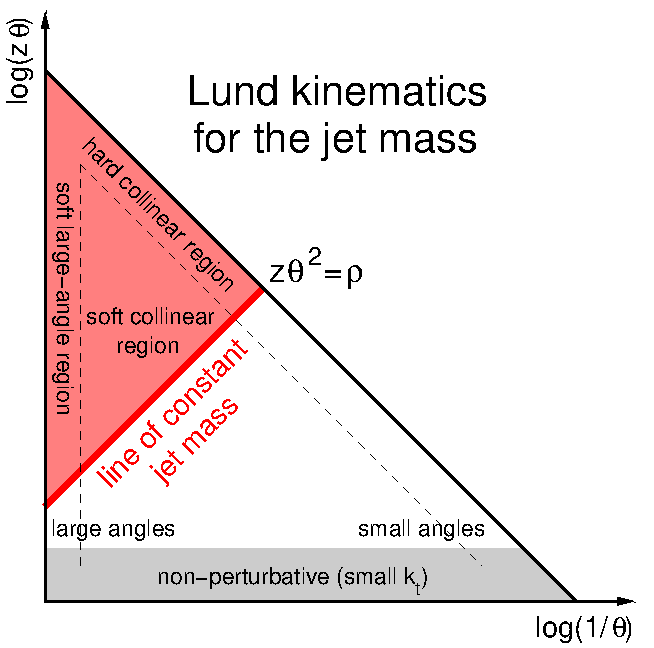
\includegraphics[width=0.45\textwidth]{figures/Lund-plain.pdf}%
 \caption{Lund diagram for the jet mass distribution at LL. The solid
   red line corresponds to emissions yielding the requested jet mass,
   \ie with $z\theta^2=\rho$ (using angles rescaled by $R$). The
   shaded red area is the vetoed area associated with the Sudakov
   suppression. ``Soft, wide-angle'' emissions have a small $k_t$ and
   angles of order $R$, and ``hard collinear'' splittings have a small
   angle and a large $z$ fraction. The shaded grey region at the
   bottom of the plot corresponds to the non-perturbative,
   small-$k_t$, region.}\label{fig:lund-plain}
\end{figure}

In order to obtain explicit resummed expressions, we have to evaluate
the integrals in Eq.~(\ref{eq:res-mass-cont}) to the required
accuracy. For instance, if we aim to NLL (in the small $R$ limit), we
have to consider the running of the strong coupling at two
loops. Furthermore, we have to include the complete one-loop splitting
function $P_q(z)$ as well its soft contribution at two loops, which
corresponds to the two-loop cusp anomalous dimension
$K=C_A \left (\frac{67}{18}- \frac{\pi^2}{6} \right ) - \frac{5}{9}
n_f$. We note that this contribution accounts for correlated gluon
emission which are unresolved at NLL accuracy. This correction can
therefore be absorbed into the running coupling, giving rise to the
so-called Catani-Marchesini-Webber (CMW) scheme~\cite{Catani:1990rr}:
\begin{equation}\label{eq:CMW} 
\frac{\as^\text{CMW}(\mu)}{2\pi }=\frac{\as(\mu)}{2 \pi}+ K \left(\frac{\as(\mu)}{2 \pi}\right)^2.
\end{equation}
%    
We write the resummed exponent as
\begin{equation}\label{eq:radiator-nll-expansion}
R (\rho)= Lf_1(\lambda)+ f_2(\lambda),
\end{equation}
where $f_1$ and $f_2$ resum leading and next-to-leading logarithms,
respectively:
\begin{equation}
\label{eq:quark}
f_1(\lambda) =  \frac{C_F}{\pi \beta_0 \lambda} \left [ \left(1-\lambda \right ) 
\log \left(1-\lambda \right)-2 \left ( 1-\frac{\lambda}{2} \right ) \log \left
  (1-\frac{\lambda}{2} \right ) \right ],
\end{equation}
and
\begin{multline} \label{eq:radiator-nll-contribution}
f_2(\lambda) =  \frac{C_F K}{4 \pi^2 \beta_0^2} \left [2 \log \left 
(1-\frac{\lambda}{2} \right ) - \log \left (1-\lambda \right )\right ] -
\frac{ C_F B_q}{\pi \beta_0} \log \left ( 1-\frac{\lambda}{2} \right ) 
\\  +\frac{C_F \beta_1}{2 \pi \beta_0^3} \left [ \log \left (1-\lambda \right )-2 \log 
\left (1-\frac{\lambda}{2} \right ) + \frac{1}{2} \log^2 \left (1- \lambda \right ) 
- \log^2 \left (1-\frac{\lambda}{2} \right ) \right ],
\end{multline}
$\lambda = 2 \alpha_s\beta_0 L$, $B_q$ was defined in
Eq.~(\ref{eq:B1}), and $\alpha_s\equiv\alpha_s\left(QR/2\right)$ is
the $\overline{\text{MS}}$ strong coupling.
% 
Since this kind of results will appear repeatedly throughout this
book, we give an explicit derivation of the above formul\ae\ in
Appendix~\ref{chap:app-analytic-details}. In the above results we have also
introduced the one-loop and two-loop coefficients of the QCD $\beta$-function, namely $\beta_0$ and $\beta_1$. 
Their explicit expressions are given in Appendix~\ref{chap:app-analytic-details}.

In order to achieve the complete NLL resummation formula for the
invariant mass distribution of narrow, i.e.\ small $R$, jets we need
to consider two additional contributions: multiple emissions and
non-global logarithms~\cite{Dasgupta:2001sh}. We have already
mentioned how to deal with the former: in the real-emission
contribution to Eq.~(\ref{eq:res-mass-start}), we can no longer apply
the strong-ordering simplification 
Eq.~\eqref{eq:strong-rho-ordering-LL} and the resummed calculation must
be done in a conjugate (Mellin) space in order to factorise the
observable definition. 
%
At the end of the calculation, the result must then brought back to
physical space. In case of jet masses this inversion can be done in
closed-form and, to NLL accuracy, it can be expressed as a correction
factor:
\begin{align}\label{eq:mult-emission-nll}
\mathcal{M}(\rho)&=  \frac{e^{-\gamma_E R'(\rho)}}{\Gamma(1 +R'(\rho))}.
\end{align}
Non-global logarithms are instead resummed into a factor $\mathcal{S}(\rho)$ which has a much richer (and complex) structure. We will discuss it in some detail in Sec.~\ref{sec:non-global}. Putting all things together the NLL result for the cumulative mass distribution reads
\begin{equation}
  \label{eq:Sigma-plain-jet-mass}
  \Sigma^{(\text{NLL})}(\rho) = \mathcal{M} \,\mathcal{S}\, e^{-R} .
\end{equation}

Thus far we have discussed the jet mass distribution in the context of perturbation theory. However, when dealing with soft and collinear emissions, we are probing the strong coupling deeper and deeper in the infra-red and we may become sensitive to non-perturbative contributions. This is clearly dangerous because as the coupling grows, perturbation theory becomes first unreliable and then meaningless. The presence of an infra-red singularity (Landau pole) for the coupling makes this breakdown manifest: at long distances we cannot use partons as degrees of freedom but we have to employ hadrons. 
%
From this point of view it is then crucial to work with IRC safe observables, for which we can identify regions in which the dependence on non-perturbative physics can be treated as a (small) correction.


\subsection{A sanity check: explicit calculation of the second order}\label{sec:sanity}
\begin{figure}[tb]
  \begin{center}
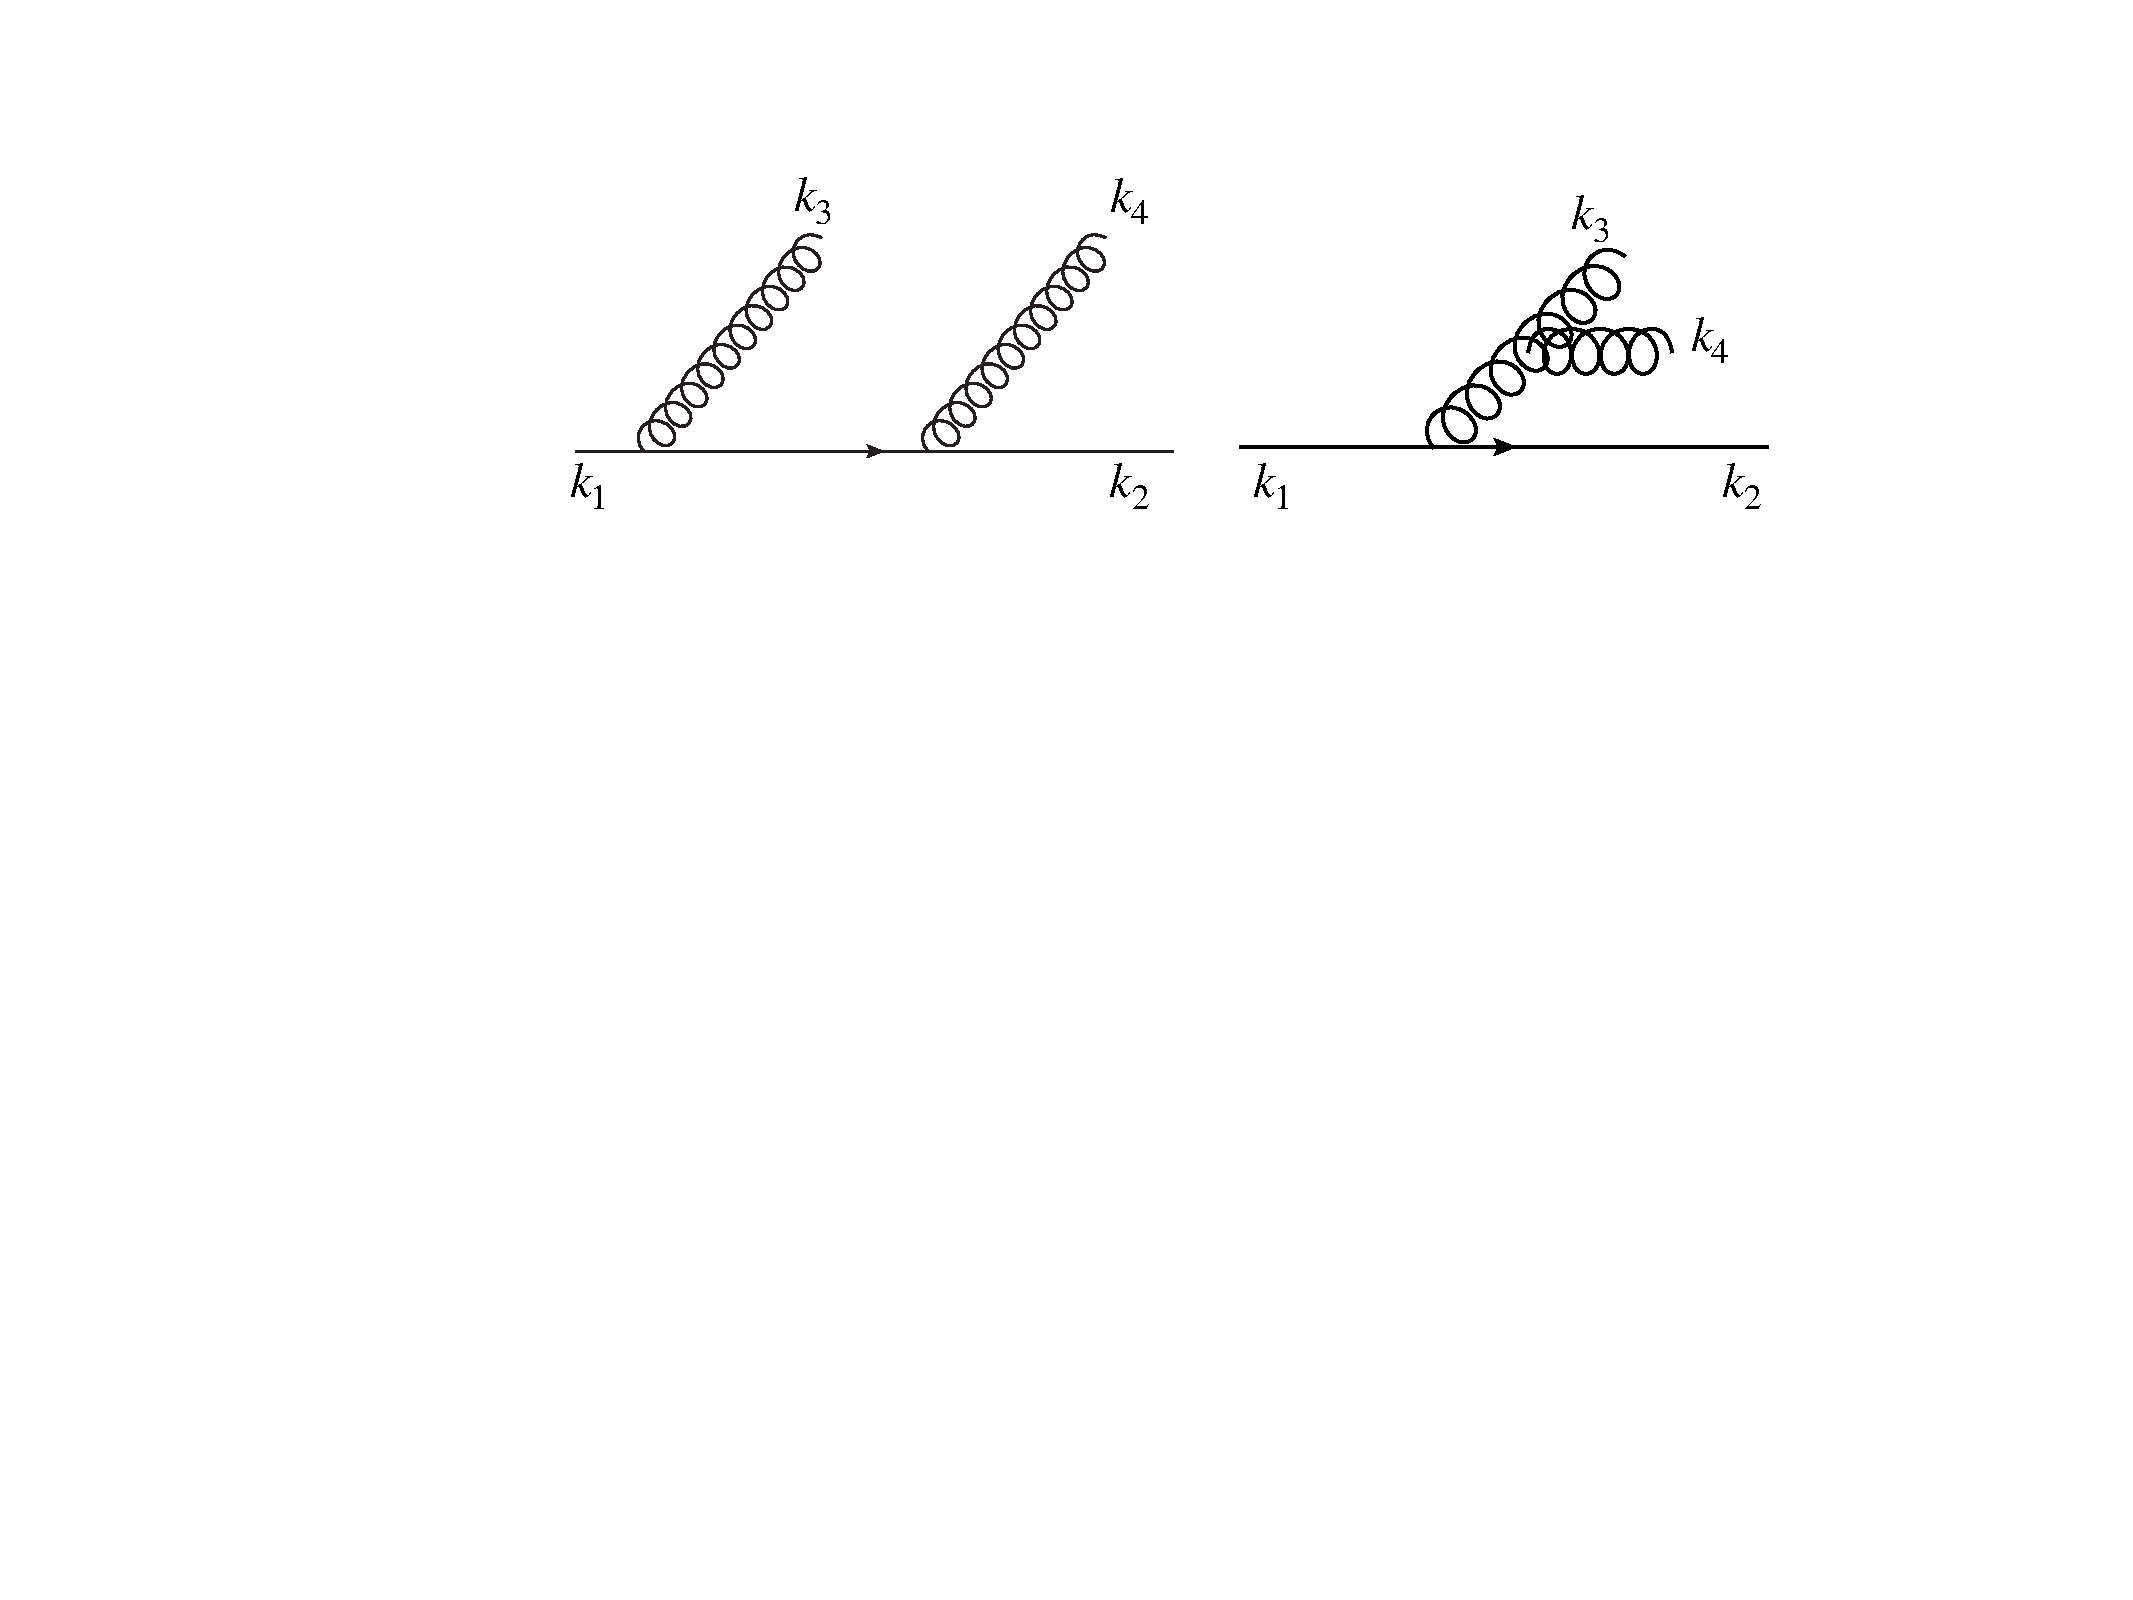
\includegraphics[width=0.8\textwidth]{figures/2gluons}
    \caption{A schematic representation of the types of contributions to the strongly order emission of two soft gluons, in the double real-emission case: independent emission  of the left and correlated emission on the right.}
    \label{fig:ind-corr}
  \end{center}
\end{figure}


As a sanity check of the all-order calculation we have performed in the previous section, we explicitly calculate the double logarithmic contribution at two loops and compare it to the expansion of the resummation to second order.
%
Thus, we need to consider the squares matrix element for the emission
of two soft gluons with momenta $k_3$ and $k_4$, off a $q \bar q$
dipole, in the limit where both $k_3$ and $k_4$ are soft, with $k_4$ much softer than $k_3$~\cite{Catani:1983bz,Dokshitzer:1992ip}. This can be written as the sum of two pieces: independent and correlated emissions
\begin{equation}\label{eq:2gluons}
W= \cf^2 W^{(\rm ind)}+ \cf \ca W^{(\rm corr)},
\end{equation}
where
\begin{eqnarray}
W^{(\rm ind)}&=&   \frac{2\, k_1\cdot k_2}{k_1\cdot k_3 \, k_2 \cdot k_3}   \frac{2\, k_1\cdot k_2}{k_1\cdot k_4 \, k_2 \cdot k_4}, \label{eq:independent}\\
W^{(\rm corr)}&=&  \frac{2\, k_1\cdot k_2}{k_1\cdot k_3 \, k_2 \cdot k_3}
 \left( \frac{k_1\cdot k_3}{k_1\cdot k_4 \, k_3 \cdot k_4}+ \frac{k_2\cdot k_3}{k_2\cdot k_4 \, k_3 \cdot k_4}-
  \frac{k_1\cdot k_2}{k_1\cdot k_4 \, k_2 \cdot k_4}
 \right).\label{eq:correlated}
\end{eqnarray}
The two contributions are schematically shown in Fig.~\ref{fig:ind-corr}.
%
Because we are interested in the $\as^2 L^4$ contribution to the cumulative distribution, which is the most singular one, we expect it to originate from the independent emission  of two gluons in the soft and collinear limit. 
%
We have to consider three types of configuration: double real emission, double virtual and real emission at one loop. 
%
For each of the three types, the contribution to the squared matrix
element for ordered two-gluon emission is the same up to an overall sign. Focusing on the independent emission contribution, the result for the double real (RR) or double virtual (VV) is
%
\begin{equation}
W^{(\rm ind)} =   \frac{256}{Q^4} \frac{1}{z_3^2 z_4^2} \frac{1}{\theta_3^2 \theta_4^2 }\,.
\end{equation}
A similar result holds for the real emission at one loop, with a
relative minus sign. The latter has to be counted twice because the real
emission could be either $k_3$ (RV) or the softer gluon $k_4$ (VR).
 %
 We are now in a position to compute the jet mass distribution at the two-gluon level for the independent emission $C_F^2$ term. 
% 
To perform this calculation we note that it is actually more convenient to consider the differential jet mass distribution rather than the cumulative, as we usually do. In fact, if we demand $m^2>0$, then the double virtual configuration does not contribute because it lives at $m^2=0$.
% 
Therefore we consider
\begin{equation}
\frac{d \tilde \sigma}{d \rho}=\frac{1}{\sigma_0}\frac{d \sigma}{d \rho}=
\as \frac{d \tilde \sigma^{(1)}}{d \rho}+\as^2 \frac{d \tilde \sigma^{(2)}}{d \rho}+ \ord \left(\as^3 \right).
\end{equation}


We start by noting that the phase space integration region for all configurations can be divided according to whether the real gluons $k_3$ and $k_4$ are inside or outside the jet of interest. We have four distinct regions: $k_3,k_4$ both outside the jet, $k_3,k_4$ both inside the jet or either of the gluons inside and the other outside the jet. The condition for a given gluon to end up inside or outside the jet depends on the jet definition. 
In the anti-$k_t$ algorithm with radius $R$ the condition is
particularly simple when considering only soft emissions: a soft
emission $k_i$ is inside the jet if it is within an angle $R$ of the
hard parton initiating the jet, otherwise it is outside. As we have already noted, the anti-$k_t$ algorithm in the soft limit works as a perfect cone.

Let us consider all four cases one by one.
%
The contribution where both $k_3$ and $k_4$ are outside the jet
trivially vanishes since it gives a massless jet.
%
We then consider the case where the harder emission $k_3$ is in the
jet and $k_4$ is out. Graphs RR and RV cancel since the real $k_4$ does not contribute to the jet mass exactly like the virtual $k_4$. This leaves diagram VR, which gives zero since the in-jet gluon $k_3$ is virtual and hence does not generate a jet mass.
%
Hence the region with $k_3$ in and $k_4$ out gives no contribution. 
%
The contribution where $k_4$ is in the jet and $k_3$ out vanishes for the same reason.
%
Hence we only need to treat the region with both gluons in the jet and
we shall show that this calculation correctly reproduces the result
based on exponentiation of the single gluon result. The sum of the RR,
RV and VR contributions can be represented as\footnote{Here with an
  abuse of notation we are indicating the LHS of the equation as
  $\as^2 \frac{d \tilde \sigma^{(2)}}{{d}\rho}$, while we really mean
  only its double leading contribution.} (with $d\Phi$ defined in Eq.~\eqref{eq:phase-space-integration})
\begin{equation}
\as^2 \frac{d \tilde \sigma^{(2)}}{{d}\rho} = \int d \Phi\, W \left[ \delta\left(\rho- z_3 \theta_3^2-z_4 \theta_4^2\right)-\delta\left(\rho-z_3 \theta_3^2\right)-\delta \left(\rho-z_4 \theta_4^2 \right) \right],
\end{equation}
%
where in order to keep our notation simple, we have switched to rescaled angular variables: $\theta_i  \to \frac{\theta_i}{R}$, so that now $\theta_i<1$.
%
To proceed, we note that in the leading-logarithmic approximation
emissions are also strongly ordered in $z\theta^2$, \ie we
have either $z_3\theta_3^3\gg z_4\theta_4^2$, or $z_4\theta_4^3\gg
z_3\theta_3^2$.
%
This means that only the largest of $z_3\theta_3^3$ and
$z_4\theta_4^2$ contributes to $\delta\left(\rho-z_3 \theta_3^2-z_4
  \theta_4^2 \right)$, with the other being much smaller. We can
therefore write
\begin{equation}\label{eq:delta-2em-simplifacation-LL}
  \delta\left(\rho-z_3 \theta_3^2-z_4 \theta_4^2\right) \to
  \delta\left(\rho-z_3 \theta_3^2\right)\Theta\left(\rho>z_4
    \theta_4^2 \right)+3\leftrightarrow 4\,.
\end{equation} 
Doing so and using the explicit forms of $W$ and the phase space $d \Phi$ in the small angle limit we get 
\begin{multline}
\as^2 \frac{d \tilde \sigma^{(2)}}{{d}\rho} = - \left ( \frac{\alpha_sC_F}{\pi} \right)^2 
\int \frac{d\theta_3^2}{\theta_3^2}\frac{d\theta_4^2}{\theta_4^2} 
\frac{d\phi}{2\pi} \frac{dz_3}{z_3} \frac{dz_4}{z_4} \left[ \delta\left(\rho-z_3 \theta_3^2\right)\Theta\left(z_4 \theta_4^2 >\rho \right)+3 \leftrightarrow 4 \right]\\ \Theta \left(z_3>z_4\right),
\end{multline}
where $\phi$ is the azimuthal angle between the two gluons (the other
azimuthal integration is trivial because the matrix element does not
depend on either $\phi_3$ or $\phi_4$).
%
We note that the overall factor
$-\Theta\left(z_4 \theta_4^2 >\rho \right)$ comes again from the
region where $k_4$ is virtual, while real and virtual emissions cancel
each other for $z_4 \theta_4^2 <\rho$.
%
Carrying out the integrals we obtain
\begin{equation}\label{eq:LL-result-alphas2}
\as^2 \frac{d \tilde \sigma^{(2)}}{{d}\rho}  = -\frac{1}{2} \left(\frac{\alpha_sC_F}{\pi} \right)^2 \frac{1}{\rho} \log^3 \left (\frac{1}{\rho} \right),
\end{equation}
which is precisely the result obtained by expanding the exponentiated double-logarithmic one-gluon result to order $\alpha_s^2$ and differentiating with respect to $\rho$.
Thus the standard double-logarithmic result for the jet-mass
distribution arises entirely from the region with both gluons in the
jet. Contributions from soft emission arising from the other regions
cancel in the sense that they produce no relevant logarithms.

We note that since we have used a soft-gluon approximation (with
gluons emitted from colour dipoles), the result above does not
include the contribution from hard-collinear splittings which, at this
order would give a contribution
$\frac{3}{2}\big(\frac{\alpha_sC_F}{\pi}\big)^2\frac{1}{\rho}\log^2(\rho)B_q$.
%
Finally, beyond the double-logarithmic approximation, the
approximation~\eqref{eq:delta-2em-simplifacation-LL} is no longer
valid. It does bring a correction to Eq.~\eqref{eq:LL-result-alphas2}
coming from the difference between the left-hand side and the right-hand side of
\eqref{eq:delta-2em-simplifacation-LL}.
%
In practice, we get
%
\begin{align}
& \frac{1}{2} \left ( \frac{\alpha_sC_F}{\pi} \right)^2 
\int \frac{d\theta_3^2}{\theta_3^2}\frac{d\theta_4^2}{\theta_4^2} 
  \frac{dz_3}{z_3} \frac{dz_4}{z_4} \left[
 \delta\left(\rho-z_3 \theta_3^2-z_4 \theta_4^2\right)
 -\delta\left(\rho-z_3 \theta_3^2\right)\Theta\left(z_4 \theta_4^2 >\rho \right)
 -3 \leftrightarrow 4 \right]\nonumber\\
  &= \left ( \frac{\alpha_sC_F}{\pi} \right)^2 
\int_0^\rho \frac{d\rho_3}{\rho_3}\frac{d\rho_4}{\rho_4} 
  \log\left(\frac{1}{\rho_3}\right)\log\left(\frac{1}{\rho_4}\right) \left[
 \delta\left(\rho-\rho_3-\rho_4\right) -\delta\left(\rho-\rho_3\right)\right]
    \Theta(\rho_3>\rho_4)\nonumber\\
  &= \left ( \frac{\alpha_sC_F}{\pi} \right)^2 \frac{1}{\rho}
\int_0^\rho \frac{d\rho_4}{\rho_4} 
  \log\left(\frac{1}{\rho_4}\right)
    \left[\log\left(\frac{1}{\rho-\rho_4}\right)-\log\left(\frac{1}{\rho}\right)\right]\nonumber\\
  &= \left ( \frac{\alpha_sC_F}{\pi} \right)^2 \frac{1}{\rho}
\frac{\pi^2}{6}  \log\left(\frac{1}{\rho}\right) + \text{(terms with no
    $\log(\rho)$ enhancements)}
\end{align}
%
where we have introduced $\rho_i=z_i\theta_i^2$ and used
$\int\frac{d\theta_i^2}{\theta_i^2}\frac{dz_i}{z_i}f(\rho_i) = \int\frac{d\rho_i}{\rho_i}\log(1/\rho_i)f(\rho_i)$.
% 
It is easy to show that this contribution corresponds exactly to the
first non-trivial correction from $\mathcal{M}(\rho)$ in
Eq.~(\ref{eq:mult-emission-nll}), after differentiation with respect to $\rho$,
with $R'(\rho)=\frac{\alpha_sC_F}{\pi}\log\big(\tfrac{1}{\rho}\big)$.

\subsection{Non-global logarithms}\label{sec:non-global}
\begin{figure}[tb]
  \begin{center}
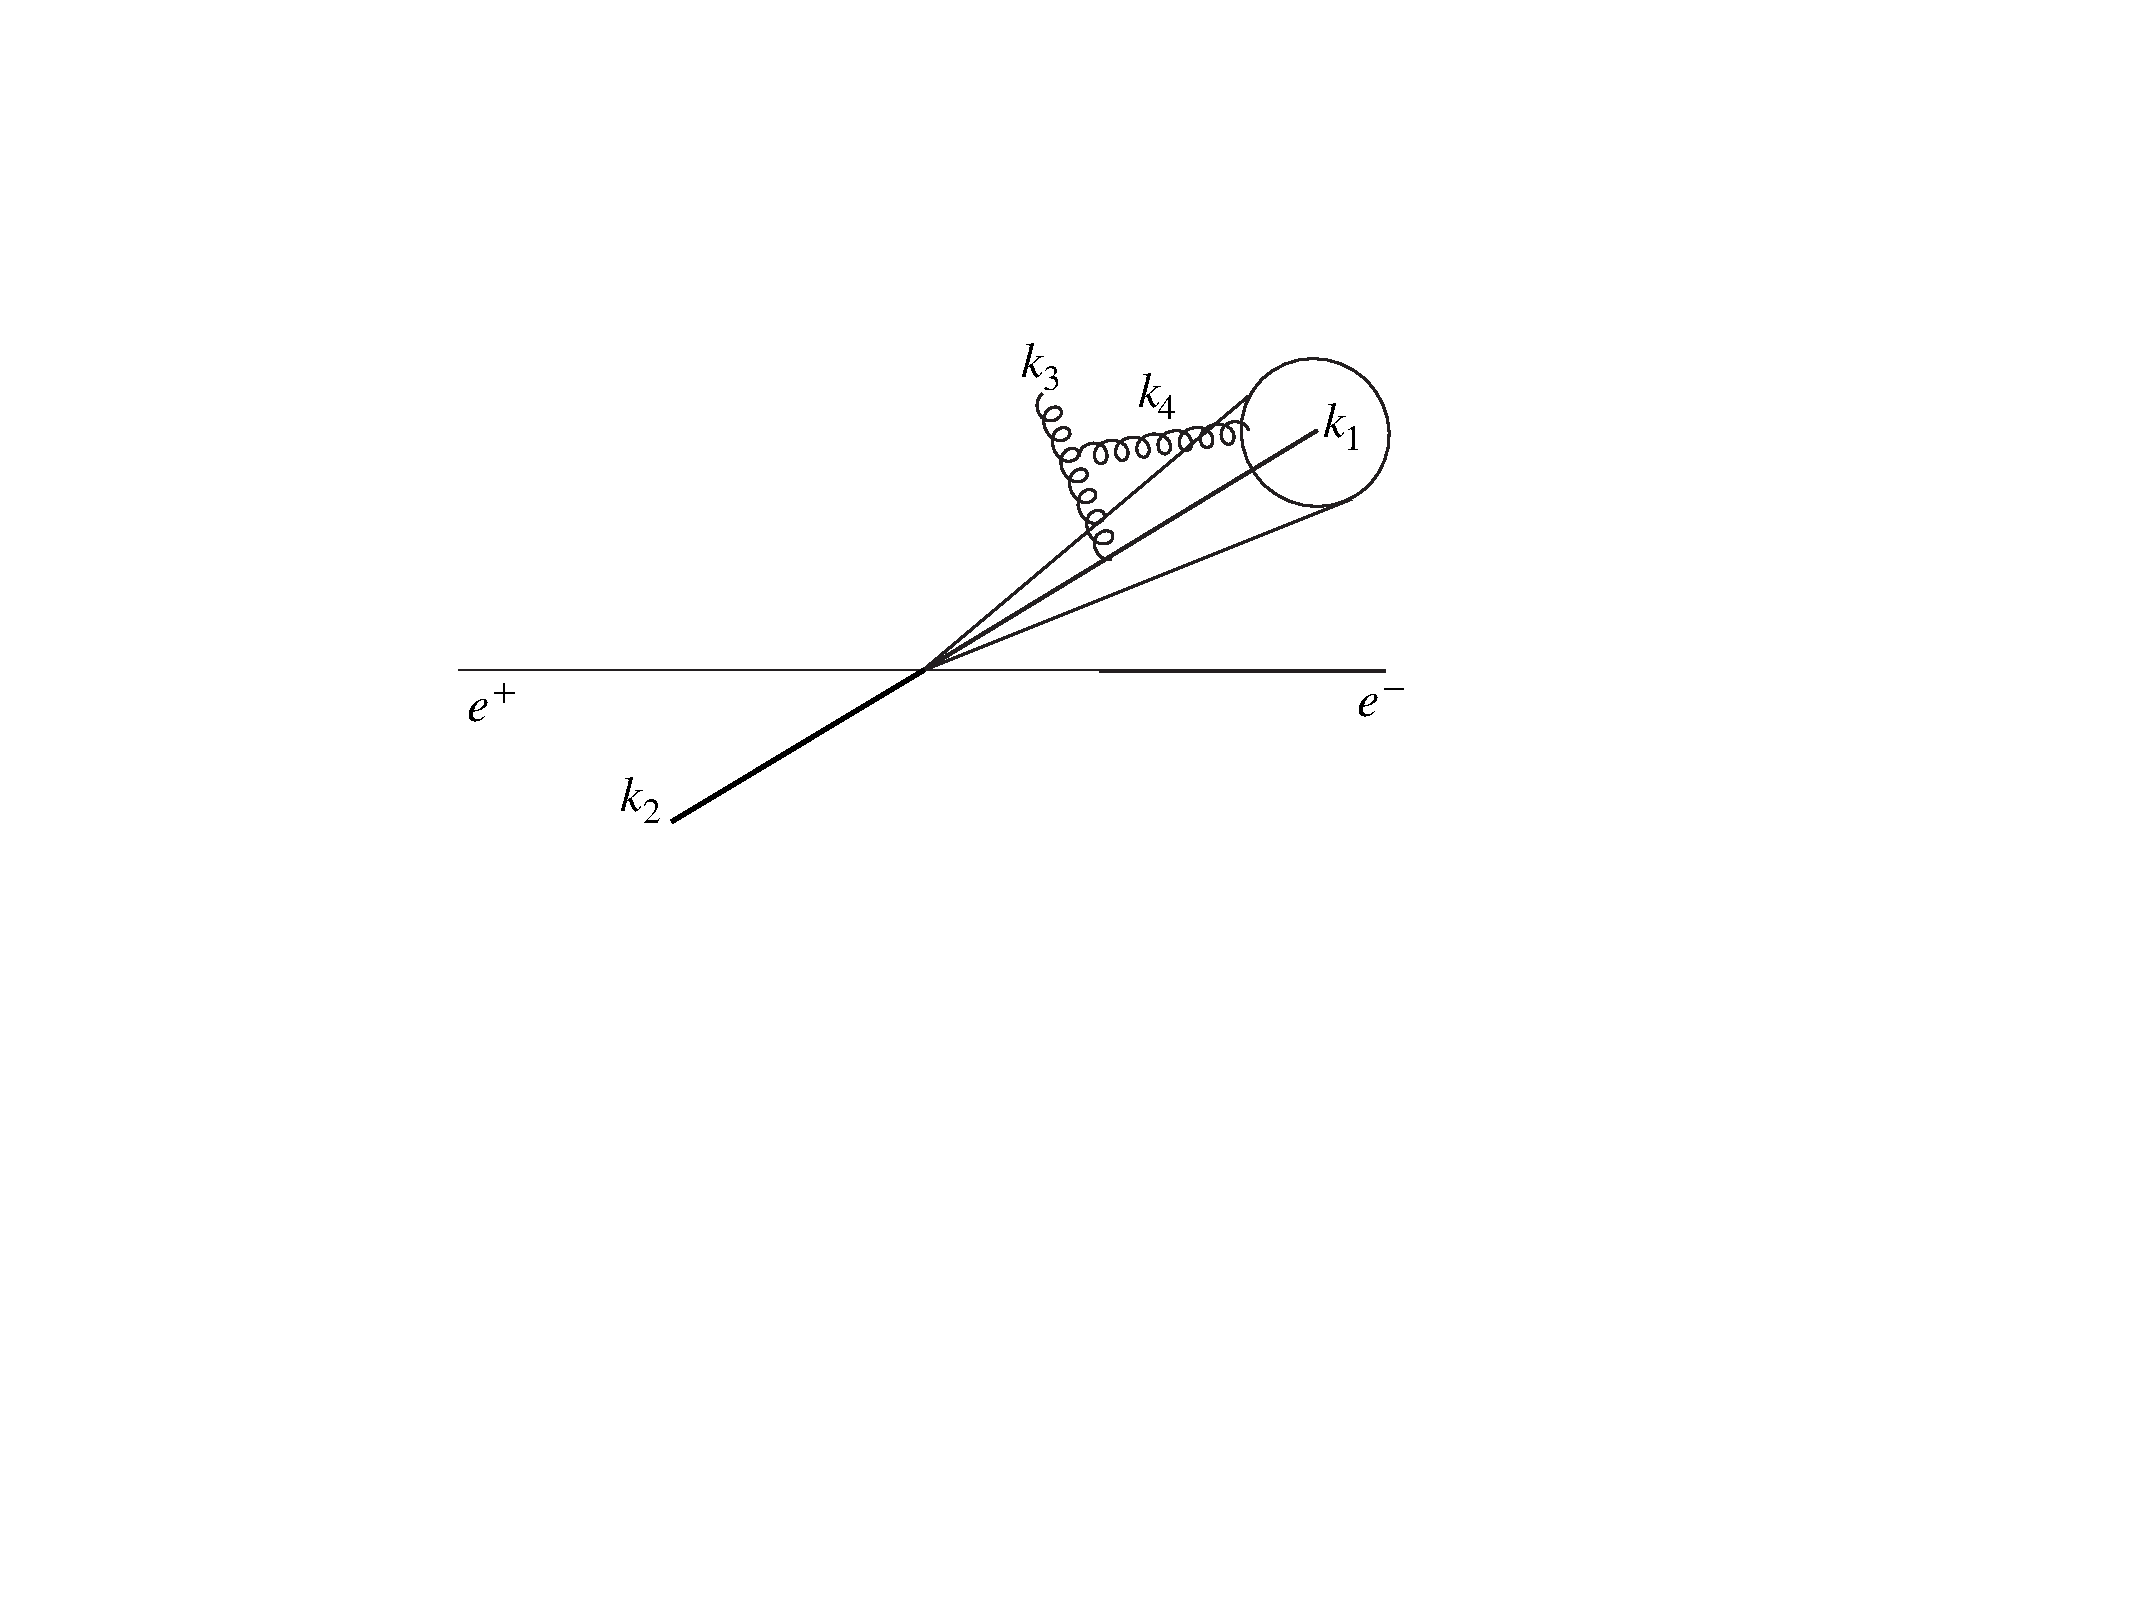
\includegraphics[width=0.7\textwidth]{figures/ngjet}
\caption{Kinematic configuration that gives rise to non-global
  logarithms to lowest order in perturbation theory. The $k_3$ gluon
  is in the jet and does not contribute to the jet mass, while the
  $k_4$ gluon is in the jet and thus contributes to the jet mass.}
    \label{fig:non-globalcontribution}
  \end{center}
\end{figure}
In Sec.~\ref{sec:jet-mass-res} we have described an all-order calculation that aims to resum large logarithms of the ratio of the jet mass to the hard scale of the process to NLL. Furthermore, in Sec.~\ref{sec:sanity} we have verified the leading logarithmic behaviour predicted by the resummation by performing a two-loop calculation in the soft and collinear limit. 
%
In order to do that we have considered the independent emission contribution to the soft eikonal current Eq.~(\ref{eq:2gluons}).
%
For observables that are sensitive to emissions in the whole phase-space, such as for instance event shapes like thrust~\cite{Farhi:1977sg} a similar exercise can be also done for the correlated emission contribution to the soft current. Then we would find that these effects are fully accounted for by treating the running coupling in the CMW scheme, i.e.\ by considering the two-loop contribution to the cusp anomalous dimensions.
%
However, it turns out that for so called non-global observables, i.e.\ observables that are sensitive only to a restricted region of phase-space, the all-order calculation previously described is not enough to capture full NLL accuracy. Indeed, correlated gluon emissions generate a new tower of single-logarithmic corrections~\cite{Dasgupta:2001sh,Dasgupta:2002bw}  the resummation of which is far from trivial.

Let us focus our discussion on a fixed-order example, which illustrates how a single logarithmic contribution arises in non-global observables. 
%
Because we are dealing with an observable that is only sensitive to emissions in a patch of the phase-space, we can have a configuration where a gluon is emitted outside this patch, in this case outside the jet, and it re-emits a softer gluon inside the jet. 
%
Thus, we consider the correlated emission contribution to the matrix
element square for the emission of two soft gluons in the kinematic
region where the harder gluon $k_3$ is not recombined with the jet,
while the softer gluon $k_4$ is. 
%
In order to better illustrate the features of the calculation, in this section we are going to retain the full angular dependence, without taking the collinear limit. 
%
This makes sense because one of the gluons is emitted outside the jet, where the collinear approximation is less justified. 
%
Note that the integration over the gluon momentum $k_3$ is sensitive
to the rest of the event and it may depend, for instance, on the way
we select the jet, the mass of which we are measuring. For example, if
we only select the hardest jet in the event, then one would have to
prevent $k_3$ from clustering with $k_2$. For simplicity, in this example, we are going to
integrate $k_3$ over the whole phase-space outside the measured jet.
%
If we restrict ourselves to a jet algorithm, such as anti-$k_t$, which works as a perfect cone in the soft limit, this condition simply translates to $ 1-  \cos \theta_3> 1- \cos R$ and $1- \cos \theta_4<1- \cos R$.
%
This situation is depicted in Fig.~\ref{fig:non-globalcontribution}.
%
% Thus, we consider the first non-global contribution to the cumulative
% distribution. After adding together real and virtual corrections, we
% obtain
At order $\alpha_s^2$, the leading non-global contribution can be
written as
\begin{align}
\as^2 S^{(2)} = & -4 C_F C_A \left ( \frac{\alpha_s}{2\pi} \right)^2 \int \frac{d\omega_3}{\omega_3} \int \frac{d \omega_4}{\omega_4} 
\Theta\left(\omega_3>\omega_4 \right)
\int d\cos\theta_3 \int d\cos\theta_4  \, \Omega(\theta_3,\theta_4)\nonumber \\ 
& \,\Theta\left(\cos \theta_3<\cos R\right)
\, \Theta \left(\cos \theta_4> \cos R \right)
 \, \Theta \left(\omega_4 Q (1-\cos\theta_4)>m^2 \right),
\end{align}
In this expression, the last $\Theta$ constraint comes from adding the
real and virtual contributions for the gluon $k_4$.
%
The angular function $\Omega$ arises after integrating the correlated
matrix element square, Eq.~\eqref{eq:correlated}, over the azimuth
$\phi$. Its expression reads~\cite{Dasgupta:2001sh}
\begin{equation}
\Omega(\theta_3,\theta_4) = \frac{2}{\left(\cos\theta_4-\cos\theta_3 \right) \left(1-\cos\theta_3\right) \left(1+\cos \theta_4 \right)}.
\end{equation}
We first perform the integration over the energies of the two gluons, obtaining 
\begin{multline}
\as^2 S^{(2)} = - 2 C_F C_A \left ( \frac{\alpha_s}{2\pi} \right)^2 
\int d\cos\theta_3 \int d\cos\theta_4  
\, \Theta\left( \cos \theta_3< \cos R\right)
\, \Theta \left(\cos \theta_4>\cos R \right)
\\
\, \Omega(\theta_3,\theta_4)\log^2\left(\frac{2m^2}{Q^2(1-\cos\theta_4)}\right) \Theta\left( \frac{2m^2}{Q^2(1-\cos\theta_4)}>1\right).
\end{multline}
We can now perform the angular integrations and express the results in
terms of our rescaled variable $\rho$. The calculation can be
simplified by noting that, since we are interested only in the NLL
contribution, we can safely ignore the angular dependence in the
argument of the logarithm.
%
We obtain:
\begin{equation}
\label{eq:sigma_NG}
\as S^{(2)} = -2C_F C_A \left (\frac{\alpha_s}{2\pi}\right)^2  \frac{\pi^2}{6}\log^2\left(\frac{1}{\rho}\right) + \dots
\end{equation}
where the dots indicate subleading contributions.  It is interesting
to observe that the coefficient of the first non-global logarithm is
independent of $R$.\footnote{This result depends on the fact that we
  have integrated $k_3$ over the whole phase-space outside the
  jet. With additional constraints on the external region, the
  coefficient of $\log^2(\rho)$ would be more complex. However, in the
  small-$R$ limit, one would always obtain $\tfrac{\pi^2}{6}$ up to
  powers of $R$.}
%
This might seem counter-intuitive at first because we might naively think that the probability for $k_3$ to emit a softer gluon inside the jet must be proportional to the jet area. However, the calculation shows that there is a nontrivial and $R$-independent contribution arising from the region where both gluons are close to the jet boundary. This results in an integrable singularity which is the origin of the $\pi^2/6$ contribution.

The result in Eq.~(\ref{eq:sigma_NG}) represents only the leading term
at the first order at which non-global logarithms appear. In order to
achieve full NLL accuracy these contributions must be resummed to
all-orders. This is highly non-trivial, even if our aim is to resum
only the leading tower of non-global logarithms needed at NLL.
%
In order to perform an all-order analysis of non-global logarithms, we must consider configurations of many soft gluons. If we restrict ourselves to considering their leading contributions, which is single-logarithmic, we can assume energy-ordering; however, no collinear approximation can be made. Thus, we have to describe how an ensemble of an arbitrary number of soft gluons, all outside the jet, can emit an even softer gluon inside the jet. 

Colour correlations make the colour algebra very complex as every
emission increases the dimensionality of the relevant colour
space. Moreover, describing the geometry of such ensembles also
becomes difficult. The approach that was taken in the first analysis
of non-global logarithms~\cite{Dasgupta:2001sh} was to consider the
large-$N_C$ limit. Colour correlations becomes trivial in this limit
because the off-diagonal entries of the colour matrices vanish. Thus,
we are able to write the matrix element square for the $n$ gluon
ensemble in a factorised way~\cite{Bassetto:1984ik} and a simplified
physical picture emerges. An emission off an ensemble of $n-1$ gluons
(plus the two hard partons) reduces to the sum over the emission off
each of the $n$ dipoles.
%
When the dipole radiates a gluon, it splits into two dipoles, originating configurations which are determined by the history of the gluon branching.
%
This can be implemented as a Monte Carlo which enables one to deal
numerically with the second above-mentioned difficulty, namely the
complicated geometry of the multi-gluon final states. This solution
was first implemented in Ref.~\cite{Dasgupta:2001sh} and subsequently
used in a number of phenomenological applications,
e.g.~\cite{Dasgupta:2002dc,Banfi:2006gy,Banfi:2008qs,Banfi:2010pa,Dasgupta:2012hg}.

The numerical impact of non-global logarithm on jet mass spectra can
be large, see e.g.~\cite{Banfi:2010pa,Dasgupta:2012hg}, and because
their treatment at NLL is only approximate, they often represent the
bottleneck to reach perturbative precision in this kind of
calculations. Remarkably, as we will discuss in
Chapter~\ref{calculations-substructure-mass}, some grooming algorithms
greatly reduce or even get rid of non-global logarithms, thus paving
the way towards an improved perturbative accuracy of jet mass distributions. 


Because of their complexity, a lot of effort has been invested in better
understanding and controlling non-global logarithms. In the rest of
this section, we highlight some of the main results for the reader
interested in a deeper exploration of non-global logarithms.
%
The resummation of non-global logarithms was formalised by Banfi, Marchesini and Smye. In Ref.~\cite{Banfi:2002hw}, they were able to derive an evolution equation, henceforth the BMS equation, which, equivalently to the Monte Carlo approach, resums the leading non-global logarithm, in the large-$N_C$ limit. 
%
It has been noted~\cite{Marchesini:2003nh} that the BMS equation has the same form as the Baliksty-Kochegov (BK) equation~\cite{Balitsky:1995ub,Kovchegov:1999yj} that describes non-linear small-$x$ evolution in the saturation regime. This correspondence has been studied in detail in Refs~\cite{Avsar:2009yb,Hatta:2009nd}, where BMS and BK were related via a stereographic projection. Because a generalisation of the BK equation to finite $N_C$ exists~\cite{JalilianMarian:1997gr,Iancu:2000hn}, the correspondence between non-global logarithms and small-$x$ physics was argued to hold at finite-$N_C$ and numerical solutions have been studied~\cite{Weigert:2003mm,Hatta:2013iba}. Very recently, this correspondence was indeed mathematically established~\cite{Caron-Huot:2015bja}. 
%
In this approach, a \emph{colour density matrix} is introduced, with the aim of describing soft radiation and an evolution equation is then derived for the colour density matrix, to all-loops, at finite $N_C$. The related anomalous dimension $K$ is  explicitly computed to one and two loops. The one-loop approximation to this evolution equation coincides with the BMS equation, once the large-$N_C$ limit is taken and it confirms on a firmer ground the results of Refs.~\cite{Weigert:2003mm,Hatta:2013iba} at finite $N_C$. More importantly, the explicit calculation of the two-loop contribution to $K$ paves the way for the resummation of non-global logarithms at higher-logarithmic accuracy, although computing solutions to the evolution equation remains a challenging task.


A different approach to the question of resumming non-global logarithms was developed in Refs.~\cite{Forshaw:2006fk,Forshaw:2008cq,Martinez:2018ffw} and applied to a phenomenological study of jet vetoes between hard jets in Refs.~\cite{Forshaw:2009fz,Delgado:2011tp}. In that context, because colour-correlations were of primary interest, the large-$N_C$ limit did not seem adequate.
%
We finish this discussion pointing out that other approaches similar in spirit was recently developed using techniques of SCET.~\cite{Larkoski:2015zka,Larkoski:2016zzc,Becher:2015hka,Becher:2016mmh,Balsiger:2019tne}


\subsection{Dependence on the clustering algorithm}\label{sec:clustering}

In all the calculations performed thus far we have always treated the constraints originating from the jet algorithm in a rather simple way.
%
Essentially, we have always drawn a hard cone of radius $R$ centred on the hard parton and considered as clustered into the jet soft emissions laying within that cone. 
%
As already mentioned, this approach is justified if we are using the
anti-$k_t$ algorithm.
%
%
However, the situation changes for other members of the generalised $k_t$
family, such as the Cambridge/Aachen algorithm or the $k_t$
algorithms. Indeed, these clustering algorithms have a distance
measure which admits the possibility of two soft gluons being the
closest pair, thus combining them before they cluster with the hard
parton.


We now revisit the two-gluon calculation described in
Sec.~\ref{sec:sanity}, this time making use of the $k_t$ clustering
algorithm. We keep the same convention for the kinematics, i.e.\ the
soft gluon momenta are labelled $k_3$ and $k_4$, with $k_4$ much
softer than $k_3$.
%
As in the previous section, we should consider either the case where
both gluons are real, or the case where one of the gluons (either
$k_3$ or $k_4$) is real and the other is virtual.

We start by considering the RR contribution in different kinematic
configurations.  Clearly, when both $k_3$ and $k_4$ are beyond an angle
$R$ with respect to the hard parton there is no contribution from
either to the jet-mass.
%
When both $k_3$ and $k_4$ are within an angle $R$ of the hard parton,
both soft gluons get combined into the hard jet and this region
produces precisely the same result as the anti-$k_t$ algorithm,
corresponding to exponentiation of the one-gluon
result.\footnote{Remember that when a soft particle clusters with a
  much harder one, the resulting object has the $p_t$ and direction of
  the harder particle, up to negligible recoil.}
%
However, when $k_3$ is beyond an angle $R$ and $k_4$ is inside an angle $R$ the situation changes from the anti-$k_t$ case. 
%
This is because the $k_t$ distance between the two soft gluons can be
smaller than the $k_t$ distance between $k_4$ and the hard parton,
in which case $k_4$ clusters with $k_3$, resulting in a soft jet along
the direction of $k_3$.
%
%
Thus, when $k_3$ is beyond an angle $R$ it can pull $k_4$ out of the hard jet since the soft jet $k_3+k_4$ lays now at angle larger than $R$ with respect to the hard parton, i.e.\ outside the jet. 
%
Therefore, this kinematic configuration results in a massless jet.
%
% 
In precisely the same angular region the VR configuration is obviously
unaffected by clustering and it does give a contribution to
$\tfrac{d\sigma}{d\rho}$. This contrasts with the anti-$k_t$ case
where the real and virtual contributions cancelled exactly at this
order.
%
Note also that the RV configuration gives no contribution (as in the
anti-$k_t$ case) because no real gluons are in the jet.
%
Finally, for the case were $k_3$ is inside the jet and $k_4$ is
outside the jet, a similar situation can happen where $k_3$ and $k_4$
are clustered first, pulling $k_4$ back in the jet. This case however
does not lead to an extra contribution because, since $k_4$ is much
softer than $k_3$, it does not affect the mass of the jet already
dominated by $k_3$.

Thus a new  contribution arises for the $k_t$ algorithm from the region where the two real
gluons $k_3$ and $k_4$ are clustered, where we only get a contribution
from the case where $k_3$ is virtual and $k_4$ is real.
%
We now carry out this calculation explicitly. 
%
% 
We work in the small-$R$ limit and consider the angles $\theta_3$,
$\theta_4$ and $\theta_{34}$ as the angles between $k_3$ and the hard
parton, $k_4$ and the hard parton and $k_3$ and $k_4$ respectively. 
%
In order to apply the $k_t$-algorithm in $e^+ e^-$, we have to compare
the distances $\omega_3^2 \theta_3^2$, $\omega_4^2 \theta_4^2$ and
$\omega_4^2 \theta_{34}^2$.
%
Now since $\theta_3^2 > R^2$, $\theta_4^2 <R^2$ and
$\omega_4\ll\omega_3$, the only quantities that can be a candidate for
the smallest distance are $\omega_4^2 \theta_4^2$ and $\omega_4^2 \theta_{34}^2$. Thus
the gluons are clustered and $k_4$ is pulled out of the jet if
$\theta_{34}<\theta_4<R$.
%
Otherwise $k_4$ is in the jet and cancels against virtual corrections, precisely as it happened for the anti-$k_t$ algorithm.

Making use of the usual rescaling $\theta \to \theta/R$, we can then write the VR contribution in the clustering region as
\begin{multline} 
\frac{ d \tilde{\sigma}_2^{\mathrm{cluster}}}{d \rho}=-4 C_F^2 \left(\frac{\alpha_s}{2\pi}\right)^2 \int \frac{d\theta_3^2}{\theta_3^2}\frac{d\theta_4^2}{\theta_4^2} \frac{d\phi}{2\pi} \frac{d z_3}{z_3} \frac{dz_4}{z_4} \delta \left(\rho -z_4 \theta_4^2 \right)\Theta(z_3>z_4) \\  \Theta\left(\theta_3^2>1\right) \Theta \left(\theta_{34}^2<\theta_4^2\right)\Theta \left(\theta_{2}^2<1\right).
\end{multline}
%
Within our small-angle approximation, we can write
$\theta_{34}^2 =\theta_3^2 +\theta_4^2-2 \theta_3 \theta_4 \cos \phi$.
%
Integrating over $z_3$ and $z_4$ and using
$t= \frac{\theta_4^2}{\rho}$ one obtains
 \begin{multline} 
\frac{ d \tilde{\sigma}_2^{\mathrm{cluster}}}{d \rho}= -4 C_F^2 \left( \frac{\alpha_s}{2\pi} \right)^2 \frac{1}{\rho} \int \frac{d\theta_3^2}{\theta_3^2} \frac{dt}{t} \frac{d \phi}{2 \pi} \log(t) \\
 \Theta \left(t>1\right) \Theta \left(\theta_3^2>1\right) \Theta\left(4 \rho t \cos^2\phi>\theta_3^2\right)\Theta \left(t \rho<1 \right).
\end{multline}
Carrying out the integral over $\theta_3^2$ results in 
\begin{multline}\label{eq:logs-clustering-interm}
\frac{ d \tilde{\sigma}_2^{\mathrm{cluster}}}{d \rho}= -4 C_F^2 \left( \frac{\alpha_s}{2\pi} \right)^2 \frac{1}{\rho} \int \frac{dt}{t} \frac{d \phi}{2 \pi} \log \left(4 \rho t \cos^2 \phi \right) \log(t) 
\\ \Theta \left(t>1\right) \Theta\left(4 \rho t \cos^2\phi>1\right)\Theta \left(\rho t <1\right).
\end{multline}
Now we need to carry out the $t$ integral for which we note
$t > \mathrm{max}\left(1, \frac{1}{4\rho\cos^2 \phi}\right)$. In the
region of large logarithms which we resum one has however that
$\rho \ll 1$ and hence $4\rho\cos^2 \phi\ll 1$.
%
At NLL accuracy we can therefore take $t>\frac{1}{4\rho\cos^2 \phi}$
and replace the $\log(t)$ factor by $\log \big(\tfrac{1}{\rho}\big)$ in~\eqref{eq:logs-clustering-interm}.
%
%
It is then straightforward to carry out the $t$ integration to get
\begin{equation} 
 \frac{ d \tilde{\sigma}_2^{\mathrm{cluster}}}{d \rho}
 = -4 C_F^2 \left( \frac{\alpha_s}{2\pi} \right)^2 \frac{1}{\rho} \log\left(\frac{1}{\rho}\right) \int_{-\frac{\pi}{3}}^{\frac{\pi}{3}} \frac{d \phi}{\pi} \log^2(2 \cos \phi) = -\frac{2\pi^2}{27} C_F^2 \left( \frac{\alpha_s}{2\pi} \right)^2 \frac{1}{\rho} \log \left(\frac{1}{\rho}\right).
 \end{equation} 
This behaviour in the distribution corresponds to a single-logarithmic $\alpha_s^2 \log^2 \big(\frac{1}{\rho}\big)$ contribution to the cumulative, which is, as anticipated, necessary to claim NLL accuracy.
%
The all-order treatment of these clustering effects is far from trivial because of the complicated kinematic configurations, which results into many nested $\Theta$ function. Therefore, from this point of view, resummation of mass spectra for jet defined with the anti-$k_t$ algorithm appears simpler. Conversely, because of these clustering effects, the jet boundary becomes somewhat blurred, resulting in milder non-global contributions. 

\subsection{Non-perturbative corrections:
  hadronisation}\label{sec:plain-mass-hadronisation}

Lund diagrams, such as the one in Fig.~\ref{fig:lund-plain}, turn out
to be particularly useful in order to determine the sensitivity of an
observable to non-perturbative dynamics. We can introduce a
non-perturbative scale $\mu_\text{NP}\sim 1$~GeV below which we enter
a non-perturbative regime. Because the running coupling in
Eq.~(\ref{eq:res-mass-start}) is evaluated at a scale that represent
the emission transverse momentum with respect to the jet, a horizontal
line $z \theta =\tilde{\mu}=\frac{\muNP}{E_J R}$  marks the boundary between
perturbative and non-perturbative dynamics (recall that
$\theta$ is measured in unit of the jet radius $R$).
%
It is then simple to calculate what is the corresponding value of the jet mass for which the integrals we have to perform have support on the non-perturbative region: we just have to work out where the line of constant $\rho$ first crosses into the non-perturbative region. This happens when $z \theta= \tilde{\mu} $ and $\theta=1$, which implies $\rho=\tilde{\mu}$.
%
Thus, this simple argument suggests that the mass distribution becomes sensitive to non-perturbative physics at 
\begin{equation}\label{eq:mass-NP-estimate}
m^2\simeq \frac{\muNP}{E_J R} E_J^2 R^2= \muNP E_J R.
\end{equation}
%
%
Note that this scale grows with the jet energy, so that even apparently
large masses, $m \gg \Lambda_\text{QCD}$, may in fact be driven by
non-perturbative physics.
%
For a $3\TeV$ jet with $R=1$, taking $\muNP = 1\GeV$, the
non-perturbative region corresponds to $m \lesssim 55\GeV$,
disturbingly close to the electroweak scale!

Experimentally jets can be thought of as a bunch of collimated hadrons
(mesons and baryons). However, we have so far considered jets from a
perturbative QCD perspective and used partons to describe their constituents. 
%
%
The parton-to-hadron transition, namely hadronisation, is a
non-perturbative phenomenon.
%
Non-perturbative corrections due to hadronisation can be treated,
within certain approximations, with analytic methods, see
e.g.~\cite{Lee:2006fn,Stewart:2014nna}. For the jet mass the leading correction turns
out to be a shift of the differential
distribution~\cite{Dokshitzer:1997ew,Salam:2001bd}. Furthermore, this type of analytic calculations can provide insights about the dependence of these corrections on the parameters of the jet algorithm, such as the jet radius~\cite{Dasgupta:2007wa}.
%
Alternatively, we can take a more phenomenological point of view and
use Monte Carlo parton showers to estimate non-perturbative
correction. For instance, we can either calculate a given observable
on a simulated event with hadrons in the final state, or stop the
event simulation before hadronisation takes place and compute the same
observable with partons. We can then take the bin-by-bin ratio of the
jet mass distribution computed with and without hadronisation as a
proxy for these corrections.
%
This is the path we are going to employ in this book to illustrate the
impact of non-perturbative corrections (both hadronisation and the
Underlying Event, which we must also include when considering hadron-hadron collisions).
%
 We will present such studies in
Chapter~\ref{calculations-substructure-mass}, where hadronisation
correction to the jet mass distribution discussed here will be
compared to the ones for jets with substructure (typically grooming)
algorithms.




\section{From $e^+e^-$ to hadron-hadron collisions}\label{sec:pp-collisions}

Thus far we have discussed the resummation of the invariant mass distribution of a jet produced in an electron-positron collision. In order to be able to perform jet studies in proton-proton collision we have to extend the formalism developed so far. A detailed derivation of the resummation formulae goes beyond the scope of this book and we refer the interested reader to the original literature, e.g.\ ~\cite{Catani:1996yz,Kidonakis:1998nf}. Here, instead we briefly sketch the issues that we have to tackle and how we can go about them.

\begin{enumerate}[label=\alph*)]
%
\item As discussed in Chapter~\ref{chap:qcd-colliders}, in proton-proton collision, we work
  in the collinear factorisation framework, Eq.~(\ref{eq:master}),
  where cross-sections are described as a convolution between a
  partonic interaction and universal parton distribution functions.
  %
  Furthermore, we need to switch to the appropriate kinematic
  variables for proton-proton collisions, namely transverse momentum,
  rapidity and azimuthal angle
  (cf.~Sec.~\ref{sec:hadron-collider-kinematics}).
  %
\item The complexity of resummed calculations increases in the case of
  hadronic process because we have to deal with many hard legs with
  colour, including the initial-state partons. As we have noted in Sec.~\ref{sec:qcd_soft_fact}, factorisation in the soft limit happens at the amplitude level and interference terms play a crucial role in the soft limit. 

As a consequence, resummed calculations that aim to correctly capture these effect must account for all non-trivial colour configuration. 
%
In particular, if we have a process that at Born level as more than two coloured hard legs, either in the initial or final state, then the one-gluon emission contribution in the soft limit Eq.~(\ref{eq:dipole-quark-antiquark}) can be generalised as follows
\begin{equation} \label{eq:sumdipoles}
W= \sum_{(ij)}\frac{\alpha_s(\kappa_{ij}) \, C_{ij}}{2 \pi} \frac{p_i \cdot p_j}{(p_i \cdot k) (p_j \cdot k)},
\end{equation}
where to avoid confusion we have labelled the momenta of the hard legs as $p_i$ (rather than $k_i)$ and $k$ is the soft gluon momentum. We note that the sum runs all over the dipoles $(ij)$, i.e.\ all pairs of hard legs $i$ and $j$ . To NLL accuracy, the running coupling in Eq.~(\ref{eq:sumdipoles}) must be evaluated at the scale $\kappa_{ij}^2= \frac{2(p_i \cdot k) (p_j \cdot k)}{(p_i \cdot p_j)}$, which is the transverse momentum of the emission with respect to the dipole axis, in the dipole rest frame. $C_{ij}$ is a generalisation of the effective colour charge, Eq.~(\ref{eq:eff-col-def}), which is not necessarily diagonal:
\begin{equation}\label{eq:effective_colour}
C_{ij}=-2 \, T_i \cdot T_j,
\end{equation}
where the colour matrices $T_i$ are not necessarily in the fundamental representation, as the gluon can be emitted off a gluon line as well.
We note that the expression above greatly simplifies in the collinear limit, where one recovers the usual colour factors $C_F$ and $C_A$. However, soft emissions at large angle do contribute beyond LL and therefore dealing with the sum over dipoles is mandatory in order to achieve NLL accuracy. 

It is possible to show that, even in the presence of many hard legs, the one-loop contribution above still exponentiates. However, one must keep track, for each dipole, of the different colour flow configurations. This results into a rather complex matrix structure in colour space~\cite{Catani:1996yz,Kidonakis:1998nf}.
%
As an example, in Sec.~\ref{sec:ISR}, we will evaluate the contribution to the jet mass distribution in $pp$ collision from a soft gluon emission emitted from the dipole made up of the incoming hard legs.


\item Finally, new sources of non-perturbative corrections arise in proton-proton collisions. Collinear factorisation assumes that only one parton from each proton undergoes a hard scattering. However, we can clearly have secondary, softer, scatterings between the protons' constituents. As we have mentioned at the beginning of this book, these multiple-parton interactions produce what is usually referred to as the Underlying Event. Furthermore, because protons are accelerated and collided in bunches, we also have multiple proton-proton interactions per bunch-crossing, leading to what we call pileup.
%
As a consequence hadronic collisions are polluted by radiation that
does not originated from the hard scattering. In the context of jet
physics this radiation has important consequences as it modifies the
jet properties, e.g.\ its transverse momentum or its mass, in a way
which is proportional to powers the jet radius $R$.
More specifically, corrections to the jet transverse momentum are proportional to $R^2$, while corrections to the jet mass exhibit a $R^4$ behaviour~\cite{Dasgupta:2007wa}.
%
Therefore large-$R$ jets are more significantly affected by these effects.

Some first-principle studies have been performed, mostly concentrating on double-parton scattering (see Ref.~\cite{Diehl:2017wew} for a recent review), however most phenomenological analyses rely on models of the underlying event which are usually incorporated in Monte Carlo simulations. These models are characterised by a number of free parameters which are determined by comparisons with experimental data with a process known as \emph{tuning}. We will come back to the numerical impact of the underlying event in Chapter~\ref{calculations-substructure-mass}, where we will discuss the ability of grooming techniques to reduce such contamination.

\end{enumerate} 

To illustrate the extra complications one has to deal with in
proton-proton collisions, we conclude this chapter by computing first
the effect of initial-state radiation and then the jet mass
distribution in Z+jet events.


\subsection{Initial-state radiation as an example}\label{sec:ISR}

In this section we sketch the calculation of the contribution to the jet mass distribution from the emission of a soft a gluon from the dipole formed by the two incoming hard legs. This can be taken as a good proxy to the effect of initial-state radiation.
%
As it is the first calculation we perform with hadron-collider
kinematic variables, let us explicitly specify the
kinematics:
\begin{align}
p_1 &= \frac{\sqrt{s}}{2} x_1 \left (1,0,0,1 \right),\quad
p_2 = \frac{\sqrt{s}}{2} x_2 \left (1,0,0,-1 \right), \nonumber \\
p_3 &= p_t \left( \cosh y, 1,0,\sinh y \right), \quad
 k=  k_t \left(\cosh \eta, \cos \phi, \sin \phi, \sinh \eta \right), 
\end{align}
where $p_1$ and $p_2$ denote the four-momenta of the incoming hard
partons, $p_3$ the momentum of the jet, and $k$ of the soft gluon. It
is understood that the jet must recoil against a system with momentum
$p_4$ (not specified above), over which we are inclusive. 
Note that we have used hadron-collider variables, \ie transverse
momenta $p_t$ and $k_t$, rapidities $y$ and $\eta$, and azimuthal
angle $\phi$, assuming without loss of generality that the jet is
produced at $\phi=0$. 
%
Provided the soft gluon is clustered with the jet, its contribution to the jet mass is
\begin{align}
m^2&=(p_3+k)^2=2 p_3 \cdot k = 2 p_t k_t \left(\cosh (\eta-y) -\cos \phi \right).
\end{align}
%
We can now write the contribution to the cumulative distribution from
the 12 dipole as
\begin{align}
\as \Sigma^{(1)}_{12} &= -C_{12} \int k_t dk_t d\eta \frac{d\phi}{2\pi} \frac{\alpha_s \left (\kappa_{12} \right) }{2 \pi} \frac{(p_1.p_2)}{(p_1.k)(p_2.k)} \Theta \left ((\eta-y)^2+\phi^2 <R^2 \right)
\nonumber \\ & \cdot \Theta \left 
( \frac{2 k_t}{p_t R^2} \left (\cosh (\eta-y) -\cos \phi \right) > \rho \right),
\label{eq:initial-state-rad-interm}
\end{align}
where the first $\Theta$ function is the jet clustering condition and
we have introduced $\rho= \frac{m^2}{p_t^2 R^2}$, analogously to the
$e^+ e^-$ case.
%
We next note that
\begin{equation}
\kappa^2_{12} =  2 \frac{(p_1.k)(p_2.k)}{(p_1.p_2 )} = k_t^2.
\end{equation}
Eq.~\eqref{eq:initial-state-rad-interm} therefore exhibits a
logarithmic enhancement at small $k_t$ as expected.
%
To isolate the leading (NLL) contribution, we can as usual just retain
the dependence of the jet mass on $k_t$ in the second line
of~\eqref{eq:initial-state-rad-interm}, and neglect the dependence on
$y$, $\eta$ and $\phi$ which produces terms beyond NLL accuracy.
%
We can then carry out the integration over $\eta$ and $\phi$ which
simply measures the jet area $\pi R^2$ and obtain
\begin{equation}
\as \Sigma^{(1)}_{12} = -C_{12} {R^2} \int_{\rho p_t}^{p_t} \frac{\alpha_s (k_t)}{2 \pi} \frac{dk_t}{k_t},
\end{equation}
where the lower limit of integration stems from the constraint on the
jet mass. 
%
The dipole consisting of the two incoming partons gives indeed rise to
a pure single-logarithmic behaviour. Since the emitted gluon is inside
the jet region, away from the hard legs constituting the dipole, there
are no collinear enhancements. Furthermore, the soft wide-angle single
logarithm we obtain is accompanied by an $R^2$ dependence on jet
radius, reflecting the integration over the jet area.

\subsection{The jet mass distribution in $pp \to$ Z+jet}\label{sec:Zjet}

\begin{figure}[tb]
  \begin{center}
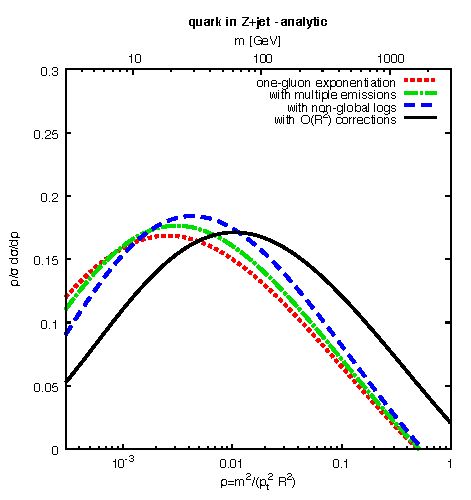
\includegraphics[page=1,scale=0.85]{figures/plain-mass.pdf}
\includegraphics[page=2,scale=0.85]{figures/plain-mass.pdf}
    \caption{The mass distribution of the quark-initiated  and gluon-initiated jets in Z+jet. The numerical impact of different contributions at NLL accuracy is shown.}
    \label{fig:z+jet}
  \end{center}
\end{figure}


We finish this chapter by showing how all the effects discussed so far affects the calculation of a jet mass distribution. 
%
We choose to study the jet mass distribution of the hardest jet produced in association with a Z boson. This process is of particular interest in the boosted regime $p_t\gg m$ or, equivalently, $\rho \ll1 $ because it is the main background for the production of a boosted Higgs boson, recoiling against the Z.
%
In practice, it also has a simpler structure than the jet mass in
dijet events since there are only three coloured hard legs.

At Born level we have to consider two partonic processes
$q g  \to Z q$ and $q \bar  q \to Z g$. 
%
We can think as the first process to describe the production of a quark-initiated jet, while the second one gives a gluon-initiated jet. We consider a very hard jet with $p_t=3$~TeV and jet radius $R=1$.
%
We plot in Fig.~\ref{fig:z+jet} the distribution of the variable
$\rho$ calculated to NLL in several approximations, on the left for a
quark-initiated jet, and on the right for a gluon-initiated one. We
start by considering  the exponentiation of the single gluon emission
Eq.~(\ref{eq:spectrum-res}), in the collinear, i.e. \ small $R$ limit
(dotted red curve). We then add the contribution to multiple
emission Eq.~(\ref{eq:mult-emission-nll}) (dash-dotted green
curve). We then add the correction due to non-global logarithms in the
large-$N_C$ limit~\cite{Dasgupta:2001sh} (dashed blue curve). Finally,
we include corrections which are suppressed by powers of the jet
radius (solid black curve).

To illustrate basic aspects of the colour algebra, we work out the
effective colour factors $C_{ij}$ associated to the colour dipoles
(cf.~Eq.~(\ref{eq:effective_colour})) of our Z+jet process.
%
Let us start with the $q g \to Z q$ process and label with 1 the
incoming quark, with 2 the incoming gluon and with 3 the outgoing
quark, we have that $T_1^2=T_3^2=C_F$ and $T_2^2=C_A$. Exploiting
colour conservation, \ie $T_1+T_2+T_3=0$ (with
all dipole legs considered outgoing), we find
\begin{equation}
%C_{12}=C_{23}=2C_A=N_C, \qquad C_{13}=2C_F-C_A=-\frac{1}{N_C}.
C_{12}=C_{23}=C_A=N_C, \qquad C_{13}=2C_F-C_A=-\frac{1}{N_C}.
\end{equation}
We then move to the gluon-initiated jet case, i.e.\ the Born process
$q \bar  q \to Z g$ and label with 1 the incoming quark, with 2 the
incoming antiquark and with 3 the outgoing gluon. We have that $T_1^2=T_2^2=C_F$ and $T_3^2=C_A$ and
\begin{equation}
%C_{12}=2C_F-C_A=-\frac{1}{N_C}, \qquad C_{13}=C_{23}=2C_A=N_C.
C_{12}=2C_F-C_A=-\frac{1}{N_C}, \qquad C_{13}=C_{23}=C_A=N_C.
\end{equation}

 We note that the $\mathcal{O}(R^2)$ corrections are rather sizeable because we are dealing with a jet with large radius. However, further corrections $\mathcal{O}(R^4)$ turn out to be very small and indistinguishable on the plot. The bulk of this large $\mathcal{O}(R^2)$ effect originates from the $12$ dipole studied above, i.e.\ it can be thought as the contribution of initial-state radiation to the jet mass. 
Finally, we remind the reader that the result in Fig.~\ref{fig:z+jet}
is not matched to fixed-order and therefore it is not reliable in the
$\rho\sim 1$ region. In particular, the resummation is not capable to
correctly capture the end-point of the distribution and matching to
(at least) NLO is mandatory to perform accurate phenomenology. 


%% GS helper for auctex
%%% Local Variables:
%%% mode: latex
%%% TeX-master: "notes"
%%% End:

%  LocalWords:  Eq eikonal NNLL NLL Catani Marchesini Webber CMW Smye
%  LocalWords:  integrable Banfi BMS Baliksty Kochegov ij eq
